\section{Sequence Information Exponent Beyond attention} \label{2506:app:sie-extra}
In the main paper, we discussed the learning of a generic Sequence Single Index model with a parametrized model like Equation~\eqref{2506:eq:model-definition}, with the goal of modelling the attention mechanism learning.
The theory of Sequence Information Exponent goes beyond this, and can be used to understand the sample complexity of the learning of a generic sequence single-index model both as a target and as a trained model.
In this Appendix, we focus on a particular choice of positional encoding that breaks the even symmetry of the model, allowing attention to weakly recover odd SIE targets. In particular, we consider a dynamical positional encoding of the form:
\begin{equation}
    P_i = \frac{c_i}{\sqrt{d}} \vec{w} + \tilde{P}_i \qquad \text{with } \tilde{P}_i\in \mathbb{R}^{L\times d} \text{ a fixed vector}.
\end{equation}
\(\vec{c}\in\mathbb{R}^L\) is a fixed vector of coefficients. We call this special version of positional encoding \textit{injected positional encoding}.
The trained model becomes:
\begin{equation} \label{2506:eq:injected-model-definition}
    f_{\vec{w}}(X) = \Pi\left[
        \SoftMax{\left(\left(X+\frac{\tilde{P}}{\sqrt{d}}\right)\vec{w}\vec{w}^\top\left(X+\frac{\tilde{P}}{\sqrt{d}}\right)^\top + \vec{c}\vec{c}^\top\right)}
    \right],
\end{equation}
and it has now a non-zero odd Hermite expansion. In Figure~\ref{2506:fig:app:extra-sie} we show examples of population losses with odd targets, learned with the model in Equation~\eqref{2506:eq:injected-model-definition}.
\begin{figure}
    \centering
    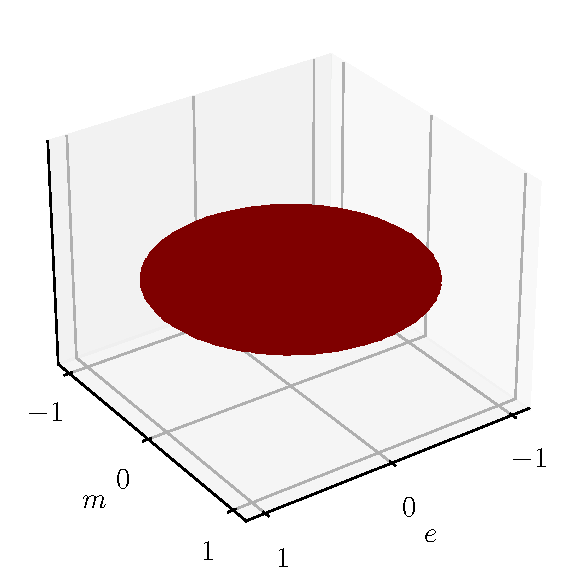
\includegraphics[width=0.22\textwidth]{figs/plot_surface/loss_surface_SIE1_peFalse}
    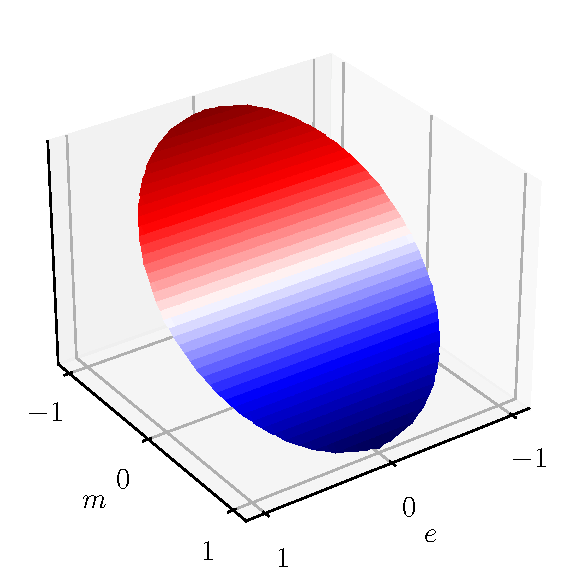
\includegraphics[width=0.22\textwidth]{figs/plot_surface/loss_surface_SIE1_peFalse_injected}
    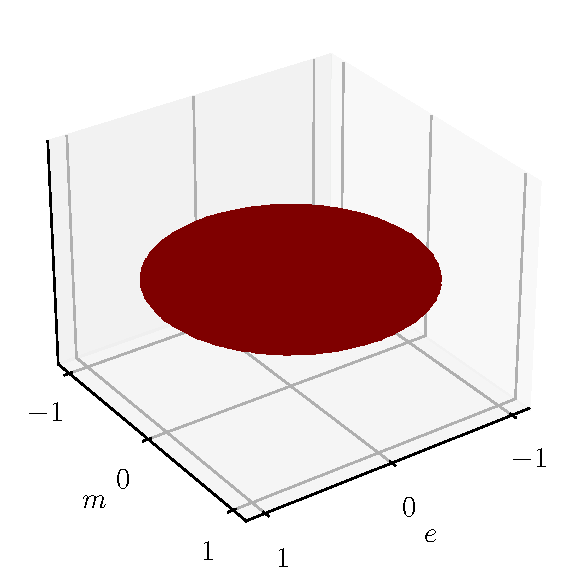
\includegraphics[width=0.22\textwidth]{figs/plot_surface/loss_surface_SIE3_peFalse}
    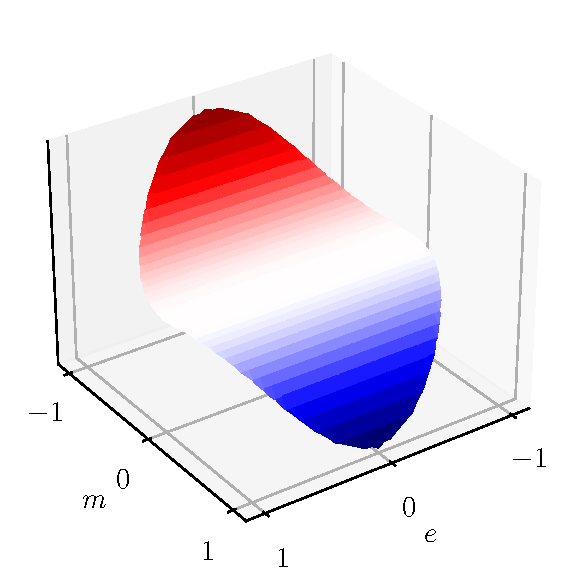
\includegraphics[width=0.22\textwidth]{figs/plot_surface/loss_surface_SIE3_peFalse_injected}
    \caption{
        Population loss of the model in Equation~\eqref{2506:eq:injected-model-definition} with odd targets.
        (left) \(g(\vec{z}_\star) = \mathrm{He}_1(\vec{z}_{\star,1}) + \mathrm{He}_1(\vec{z}_{\star,2})\), no positional encoding;
        (center-left) \(g(\vec{z}_\star) = \mathrm{He}_1(\vec{z}_{\star,1}) + \mathrm{He}_1(\vec{z}_{\star,2})\), injected positional encoding;
        (center-right) \(g(\vec{z}_\star) = \mathrm{He}_3(\vec{z}_{\star,1}) + \mathrm{He}_3(\vec{z}_{\star,2})\), no positional encoding;
        (right) \(g(\vec{z}_\star) = \mathrm{He}_3(\vec{z}_{\star,1}) + \mathrm{He}_3(\vec{z}_{\star,2})\), injected positional encoding.
        \(L=2\), \(\tilde{P} = 0\) in order to isolate the effect of the injection.
    }
    \label{2506:fig:app:extra-sie}
\end{figure}
The injected positional encoding breaks the symmetry, as the population risk plots show.
